% This is samplepaper.tex, a sample chapter demonstrating the
% LLNCS macro package for Springer Computer Science proceedings;
% Version 2.20 of 2017/10/04
%
\documentclass[runningheads]{llncs}
%
\usepackage{graphicx}
\usepackage{hyperref}
\usepackage{parskip}
% Used for displaying a sample figure. If possible, figure files should
% be included in EPS format.
%
% If you use the hyperref package, please uncomment the following line
% to display URLs in blue roman font according to Springer's eBook style:
% \renewcommand\UrlFont{\color{blue}\rmfamily}

\begin{document}
%
\title{Detachment of Pakistan from Russia-Ukraine Crisis explained via Game-Theoretic Analysis}
%
%\titlerunning{Abbreviated paper title}
% If the paper title is too long for the running head, you can set
% an abbreviated paper title here
%
\author{Mustufa Usman $|$ mu06166, Asad Raza $|$ ar06246 \\
Khubaib Sattar $|$ ks05762, Muhammad Mehdi $|$ mm05509}
% First names are abbreviated in the running head.

\titlerunning{CS-363 | Spring 2022}
\authorrunning{CS-363 | Spring 2022}

\institute{\textbf{Dhanani School of Science and Engineering, Habib University, Block 18, Gulistan-e-Jauhar, 25290, Karachi, Pakistan}\\
\email{\{mu06166, ar06246, ks05762, mm05509\}@st.habib.edu.pk}}
%
\maketitle             % typeset the header of the contribution
%
\begin{abstract}
Game Theory may be viewed as a technique for evaluating the strategic behavior of interacting and interdependent components. As a result of the ongoing Russian invasion of Ukraine, global relations are under a great deal of strain; the globe appears to be divided into nostalgic polar blocs. A great deal of pressure has been placed on Pakistan to denounce Russia for its invasion of Ukraine, but Pakistan has always maintained a position of neutrality, even so far as to abstain from voting against Russia. Implementing game theory models include elementary asymmetric deterrence and escalation games. Understanding why Pakistan has opted to detach, what benefits it involves for Pakistan, and whether or not it is generally prudent to move against the west bloc in favor of the newly formed Asian Bloc is necessary. This choice was taken after weighing several aspects (— for example, the economy and national security). Using the hawk-dove dichotomy to comprehend the current stressful situation and to identify Pakistan's crucial role in managing the current global crisis.

\keywords{Game theory  \and Russia \and Ukraine \and Pakistan \and Deterrence \and Escalation}
\end{abstract}
%
%
%
\section{Introduction}
Game Theory can be thought of as a tool for analyzing the strategic behavior of components that interact and are interconnected. With the recent ongoing Russian invasion of Ukraine, a lot of stress has been induced in global relations throughout; the world seems to be divided into nostalgic polar blocs like old times. It is apparent that the advent of this conflict will cause economic and political struggles throughout the world. Our report aims to implement game theory in order to  understand what and how each player (countries) will find the strategies that will best benefit them. The report would explore several ways to explore the cost-benefit analysis for each player in the game based on the foreign assistance, aid, economic sanctions and global prestige. The game would explore scenarios  with various numbers of players (including Pakistan, Nato Countries, and Russia). Our prime  focus would be to understand the dominant strategy for Pakistan regarding its detachment from the ongoing crises and to study the change in equilibrium with the introduction of an exogenous  change in parameter or to come up with a dynamic model that describes endogenous processes of change. Models looking forward to implementing; Classic Rudimentary Asymmetric Deterrence Game, Perfect Rudimentary Asymmetric Deterrence Game, Asymmetric Escalation Game and the Hawk-Dove Game (aka Chicken Game).

\section{Background and Scope}
Even yet, the foundations of modern game theory were laid in the United States during the Cold War, Military planners and demilitarize advocates alike relied on game theory for assistance in their discourse on the disposition of rational thinking, conflict and cooperation in the nuclear age.\\
The Russian invasion of Ukraine is a defining moment in world history, comparable to the United States' overture to China, Established in the early 1970s and the Soviet Union's disintegration in 1991, among other events. The scenario is becoming more problematic. There are several unknowns, such as how the situation may affect Russia itself. There is no doubt about its significance, but there is no indication of where it is going. If this development continues, Pakistan should really be alarmed as to what it entails for the future of this country. In order to study Pakistan's detachment from the Russia-Ukraine crisis, we would be looking and considering the following game theoretical models in our research paper:
\begin{center}
    
\textbf{a) Classic Rudimentary Asymmetric Deterrence Game}\\
\textbf{b) Perfect Rudimentary Asymmetric Deterrence Game}\\
\textbf{c) Asymmetric Escalation Game}\\
\textbf{d) Hawk-Dove Game aka Chicken Game}

\end{center}

To explain these models further in detail: 
\subsubsection{a) Classic Rudimentary Asymmetric Deterrence Game:} When nuclear weapons were first created, the belief that all possible possibilities were better than war seemed logical. State A and State B each have two actors and three possible outcomes: 1-) status quo 2-) A wins and 3-) conflict (see Fig.1 linked below). \\

\begin{center}
    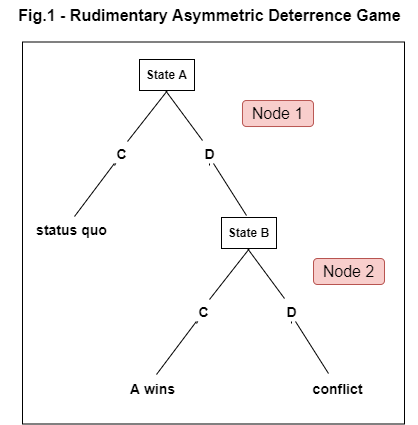
\includegraphics[width=9cm]{Asymmetric_deterrance_game.png}
\end{center}

Relatively speaking, the game of one-on-one deterrence can be described as an example of an asymmetrical or one-sided deterrence situation. Classical deterrence theory is predicated on the premise that a conflict is the worst conceivable outcome and that the participants are motivated by their own interests.
If conflict is believed to be the worst conceivable consequence, an instrumental ration can be calculated using a process known as backwards induction. Because it desires to keep things as they are, State A will logically choose for Option D even if it requires to be deterred from doing so. According to traditional deterrence theory, deterrence is logically ineffective because of two key assumptions. Deterrence theory's two basic assumptions, if viewed as a whole, do not support the theory's ability to succeed. State B has little choice but to accept defeat, as it is assumed that A's victory is more desirable.

Here, Node 1 of the game is where State A makes its first decision between cooperating with the status quo or defecting (D) and demanding that it be modified. If A choose C, the game is over and the result would be attaining status quo. State B must make a decision at node 2 if it would accept (C) or reject (D) the demand of State A, which might result in a conflict.

\newpage
\subsubsection{b) Perfect Rudimentary Asymmetric Deterrence Game:}
Classical deterrence theory has a severe empirical challenge because of the discrepancy between these two key assumptions as well as the durability of attaining status quo.
A party (such as State B) can persuade the other (like State A) that it does in fact, defect to node 2 and carry out an irrational threat by seeming to be irrational. Counter-intuitively, the participants in perfect deterrence theory are assumed to be rational at all times. It does away with the notion that a nuclear or non-nuclear deterrent meeting will invariably result in conflict.\\
Players may or may not choose to carry out a deterrent threat under perfect deterrence theory.\\
Quote - \href{https://csdp.princeton.edu/people/christopher-h-achen} {Christopher Achen} argues that “far from leaning too heavily on rational choice postulates, ‘rational deterrence theory’ necessarily assumes that nations are not always self-interestingly rational.” -Unquote

\raggedbottom

\subsubsection{c) Asymmetric Escalation Game:} To understand the protracted deterrence conflicts, more complex game models are required, such as the basic asymmetric deterrence game, which is valuable for proving the relevance of credibility and capacity. In an attempt to keep a challenger from harming a third party entity, the protégé, an actor known as the defender uses extended deterrence.
The asymmetric escalation game was devised by \href{https://arts-sciences.buffalo.edu/political-science/faculty/department-faculty/frank-c-zagare.html}{Frank Zagare} and \href{https://www.wlu.ca/academics/faculties/faculty-of-science/faculty-profiles/d-marc-kilgour/index.html}{D. Marc Kilgour} to analyze scenarios like these.
In the asymmetric escalation game, the defender's reaction options are more diverse: at decision node 2, the defendant can yield (C), it can reply in like (D), or it can escalate (E).
Nodes 3a and 3b are options for the challenger, depending on whether the defending party chooses to escalate or counter-escalate first. A counter-escalation is possible at node 4 if the challenger goes up first. Fig.2 (attached below) provides a visual representation of the possible outcomes of the asymmetric escalation game.


\begin{center}
    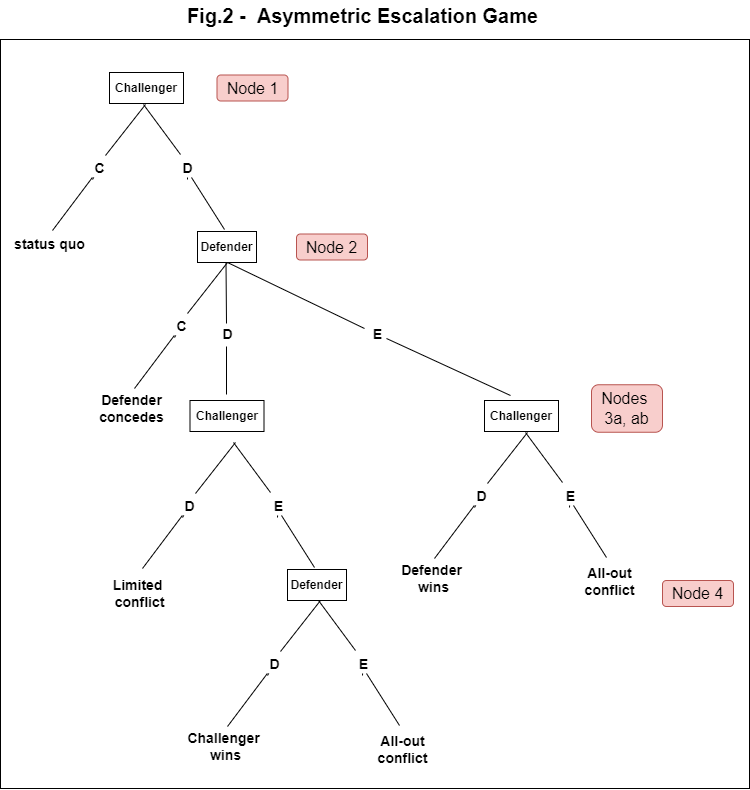
\includegraphics[width=13cm]{Asymmetric_escalation_game.png}
\end{center}

\subsubsection{d) Hawk-Dove Game aka Chicken Game:}
Consider the following scenario: 2 automobiles are competing in a race where they are driving straight against each other. The player who deviates first from the path to avoid an accident is designated as the 'Chicken,' and that player loses the game. The car that stays in the race and achieves the biggest potential profit is the winner and collects the most revenue (3). In this case, the 'hen' will obtain a one-time payout of 1 because he/she has been of assistance in preserving her own life. When both "cooperate" and escape the blow at the very same instant, each obtains a return equal to two times their initial investment. If both agents continue in the course (which is logical given their determination to win), each party receives a payout of 0. They are either dead or critically injured as a result of the head-on collision.\\\\\\\\
When one considers the Chicken Game scenario, it is natural for one to focus on the pure strategies of the Nash equilibrium, where it has been proven that the optimal rational situation that the players can reach is when one player finishes by refusing to cooperate and initiating a nuclear attack launch, while the other player cooperates, that is, it does not launch retaliatory attacks or chooses fewer desperate measures to address the situation. See Fig.3 attached below:

\begin{center}
    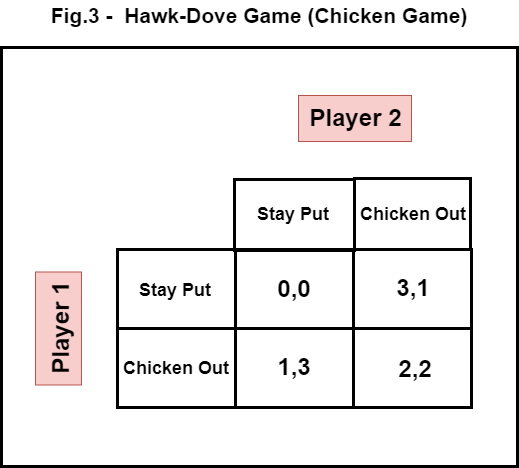
\includegraphics[width=8cm]{chicken_game (Final).png}
\end{center}

\section{Application to Contextualized Case Study}
\subsubsection{a - b) Classic / Perfect Rudimentary Asymmetric Deterrence Game:}
As a result of the Ukrainian Revolution of Dignity in 2014, Russia invaded Ukraine on February 24, 2022, resulting in a precipitous expansion of the Russo-Ukrainian War, which commenced in 2014.
A significant military buildup near Russia's border with Ukraine officially began, with up to 190,000 troops and their equipment being stationed there. Russian President Vladimir Putin also claimed that the North Atlantic Treaty Organization (NATO) posed a threat to Russian national security because it had extended towards east since the early 2000s, a claim that NATO denied. Putin demanded that NATO cease its east expansion and indefinitely bar Ukraine from ever entering the coalition.\\

Using a game theoretical framework to examine this invasion in Ukraine, we can see the aggregator or Russia's benign State A guiding the situation into conflict, when it might have chosen to maintain the status quo. Ukrainian officials should have chosen to accept the terms of a cease-fire because, according to Classical deterrence Theory, complete war is the least desirable pay-off and must be avoided at all costs. However, when viewed through the lens of Perfect Asymmetric Deterrence Theory, Ukraine's reaction is understandable; nevertheless, when a rational actor chooses an irrational strategy, conflict and the eventual outcome of an all-out war are also the possibilities that should be addressed.\\
See Fig.4 attached below:

\begin{center}
    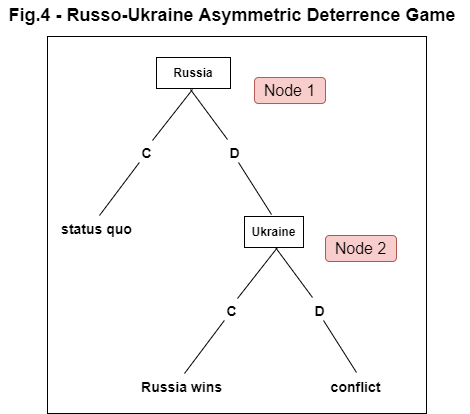
\includegraphics[width=10cm]{russia_1.png}
\end{center}

Backward induction may be used to determine what a realistic Ukrainian would do at selection node 2, and then Russia's rational option at node 1. With regard to node 2, Ukraine has an option between giving in to Russian demands and resisting them, which will lead to confrontation. Ukraine's sole choice in this situation is a surrender since fighting is thought to be the worst conceivable conclusion and Russia's success is believed to be preferable. Recognizing and aiming to eliminate the discrepancy, we by contrast maintain the rationality assumption while allowing the threat to be carried out based on probabilities.\\
Let's take a look at Pakistan's detachment from the Russia-Ukraine crisis. However, Pakistan refrained from voting against the UN General Assembly's March 2 2022 resolution that necessitates Russia to right-away, withdraw from Ukraine. It's important for governments to maintain their links with all parties concerned. United Nation Council's resolution condemning Russian aggression against Ukrai-ne was abstained from by Pakistan, an important non-NATO associate of the United States. While avoiding specific references to Russia as the perpetrator in the conflict, Foreign Minister Shah Mahmood Qureshi, alongside the Prime Minister of Pakistan - Imran Khan have repeatedly underlined that conflict is in no state's interest and a solution must come via diplomacy. A discussion with Voice of America, Shah Mahmood Qureshi clarified Pakistan's stance on the Ukraine crisis as: "We don't want to be part of any camp. We have paid the price for being in camps. That is why we are very carefully treading. We don’t want to compromise our neutrality, and that’s why we abstained.” \\
From a game-theoretical perspective, we may identify NATO as state 1 in general voting. Choosing to conduct a vote as to whether to abstain or condemn Russia, it may have decided to maintain the status quo. In a similar manner, Pakistan might be left with the option of either voting in favor of or abstaining from the resolution. Even though Pakistan's decision to abstain would have irritated the Western bloc and worsened the relations with Russia, China, and other Asian countries, the country was ready to take that risk, as though selecting the lesser of two evils through diplomacy. Classical Asymmetric Deterrence Game model and Perfect Asymmetric Deterrence Game model explain why Pakistan, a reasonable participant, chose to abstain from voting, despite its criticism of and closeness to Russia.

\subsubsection{c) Asymmetric Escalation Game:}
Ukraine has requested assistance from the West, namely the United States and NATO partners, on a number of occasions in its conflict with Russia. Though they have a great deal of war experience and competence, NATO and the United States first appeared apprehensive. Europe, on the other hand, seemed to be pushing for military intervention.\\
President of Ukraine - Volodymyr Zelenskyy has begged the United States and its allies for a no-fly zone since February 28. The Ukrainian leader added, “We repeat every day: ‘Close the sky over Ukraine!’” the Ukrainian leader said. “Close it for all Russian missiles, Russian combat aircraft, for all these terrorists. Make a humanitarian air zone—without rockets, without air bombs.” \\

This has been ruled out by NATO, fearing a full-fledged war in Europe. A no-fly zone would allow US and NATO pilots to fire down Russian jets and planes, and maybe troops on the ground as well. Experts worry that such a move might spark a catastrophic nuclear war. Assuring that no forces in the region will be dispatched to Ukraine, US President Joe Biden has consistently denied requests for a no-fly zone.\\

Experts also caution that sustaining a no-fly zone over Ukraine would be costly. Since WWII, the US military has had complete control over the sky, and has imposed no-fly zones previously. Unlike in Iraq, Bosnia and Herzegovina, and Libya, Russia possesses one of the Europe's greatest air forces, and modern armament and defense systems, increasing the risk in the overall pay-off.\\

When faced with a scenario like this, when a fault may be extremely costly, most governments choose a mild defect, such as implementing sanctions against Russia. The reason why NATO partners, including the United States, opted to implement sanctions rather than military strikes despite the possibility of Russian defeat is that they are concerned about the escalation of the conflict, which would eventually benefit no one at all.\\\\
See Fig.5 attached below:

\begin{center}
    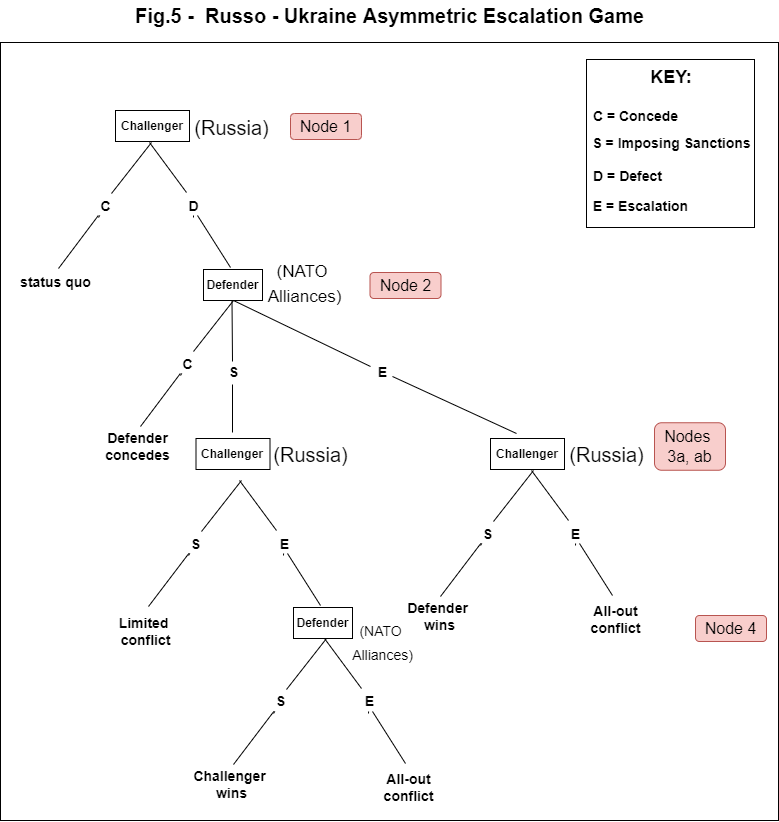
\includegraphics[width=11cm]{russo_escalation.png}
\end{center}

Pakistan is attempting to distance itself from the Russian-Ukrainian crisis. In order to retaliate against Russia, major countries were required to implement sanctions and break away economic connections with the country in some way or another. Maintaining commercial relations is essential for Pakistan. Joining the Asian Bloc, Pakistan should have strong ties with both Russia and Ukraine in order to use its strategic location as a vital gateway into the CAS countries to increase trade and economic growth. Disrupting Pakistan's diplomatic relationships would not have been beneficial to the country. In the wake of Russia's sanctions, the globe was put in jeopardy. The petroleum industry was badly affected, with the sanctions having a knock-on effect on the countries that implemented them. When Pakistan was placed in an escalation game in which it could have preferred between maintaining the status quo, imposing sanctions, or engaging in an all-out conflict with Russia, it probably made the right decision to abstain, preserving the status quo for all of the key players in the game.
\\\\
See Fig.6 attached below: 

\begin{center}
    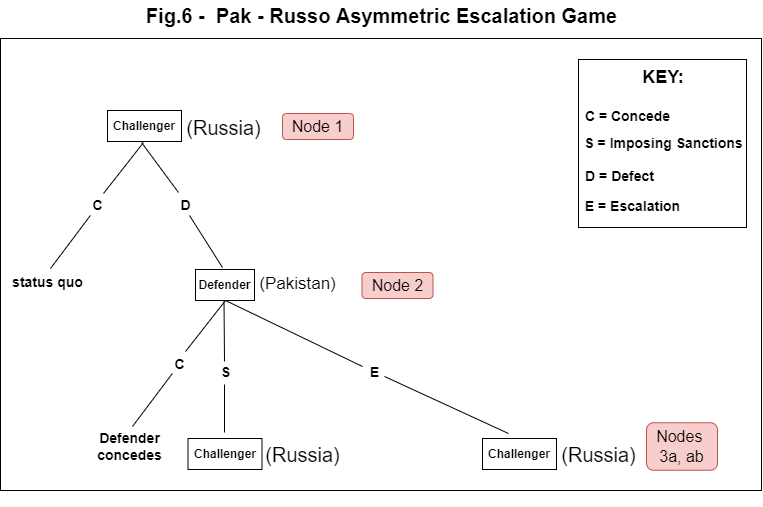
\includegraphics[width=11cm]{russo-pak.png}
\end{center}

\subsubsection{d) Hawk-Dove Game aka Chicken Game}

As Ukraine has been able to withstand Russian offensives from the outbreak of the Russian-Ukraine Crisis, it has stunned the world by taking on one of the world's superpowers. Since the beginning of the war, Russia has been unambiguous in its position on Ukraine, stating that it will not withdraw until it achieves success and that any other intervention by any country, whatsoever, would be considered an act of war and would be met with an appropriate response, along with the possibility of nuclear war. Putin authorized the Russian Nuclear Forces to enter a "special regime of combat duty" on Sunday, February 27, 2022, in accordance with the Russian Constitution. However, after the end of the cold war, all threats between superpowers have been evaluated and declared credible and capable, resulting in a slew of penalties being levied against Russian officials. This is how the west has planned to weaken Russia while avoiding direct conflict by getting stuck in a Chicken game with deteriorating economies and nuclear threats to see who would chicken out first and leave the other one alone. The sanctions have had an impact on the economies and global wealth in general.
Pakistan, on the other hand, was negatively influenced by the sanctions, but by opting to abstain, it has pulled out of the race much sooner than other countries. It was in no position to challenge in a nuclear or economic race with a powerhouse like Russia, it chose to withdraw from the situation by feigning disinterest in the Russo-Ukraine crisis.

\begin{center}
    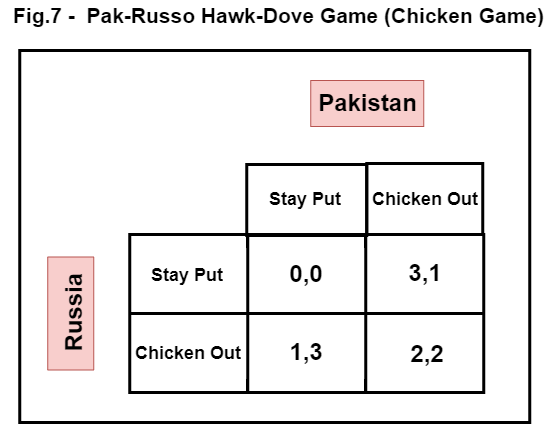
\includegraphics[width=9cm]{russo-pak-chicken.png}
\end{center}

\section{Conclusion}

The Russian-Ukrainian crisis has been a continuing struggle since 2014, and it is expected to reach its culmination in 2022. It has had a significant influence on many lives and nations, and most significantly, it has left the world peace in shreds. In a difficult situation, Pakistan was forced to choose an encampment, much like it had done in the past. However, through Asymmetric Deterrence, Escalation, and the Chicken game, we have seen and understood why Pakistan had to detach itself from the crises at hand, and maximise its payoff in the end. Strongly supporting or condemning might have gotten us into the spotlight, but it also put a lot of factors like the economy and national integrity at risk.

\begin{center}
    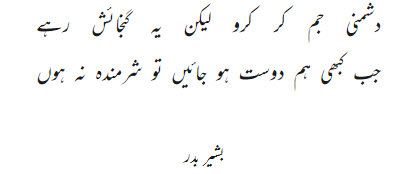
\includegraphics[width=10cm]{sher.png}
\end{center}

\newpage
\begin{thebibliography}{8}
\bibitem{ref_article1}
"Putin’S Game Of ‘Chicken’ In Ukraine". The Loop, 2022, \href{https://theloop.ecpr.eu/putins-game-of-chicken-in-ukraine/}{https://theloop.ecpr.eu/putins-game-of-chicken-in-ukraine/}

\bibitem{ref_article1}
"Game Theory: Modeling Interstate Conflict" 2022, \href{https://www.researchgate.net/publication/265353915_Game_Theory_Modeling_Interstate_Conflict}{2022, https://www.researchgate.net/publication/265353915_Game_Theory_Modeling_Interstate_Conflict}

\bibitem{ref_article1}
"Pakistan-Ukraine. Analogies in the Triangles of Regional Security Complexes". 2020, \href{https://edizionicafoscari.unive.it/media/pdf/article/annali-di-ca-foscari-serie-orientale/2020/56/art-10.14277-AnnOr-2385-3042-2020-56-009.pdf}{https://edizionicafoscari.unive.it/media/pdf/article/annali-di-ca-foscari-serie-orientale/2020/56/art-10.14277-AnnOr-2385-3042-2020-56-009.pdf}

\bibitem{ref_article1}
"Survival Politics: Assessing Pakistan’S Neutrality In The Ukraine Crisis – South Asian Voices". South Asian Voices, 2022, \href{https://southasianvoices.org/survival-politics-assessing-pakistans-neutrality-in-the-ukraine-crisis/}{https://southasianvoices.org/survival-politics-assessing-pakistans-neutrality-in-the-ukraine-crisis/}

\bibitem{ref_article1}
"Pakistan Walks Thin Line Between Russia, Ukraine" 2022, \href{https://www.voanews.com/a/pakistan-walks-thin-line-between-russia-ukraine-/6469614.html}{https://www.voanews.com/a/pakistan-walks-thin-line-between-russia-ukraine-/6469614.html}

\bibitem{ref_article1}
"Why Has Russia Invaded Ukraine And What Does Putin Want?". BBC News, 2022, \href{https://www.bbc.com/news/world-europe-56720589}{https://www.bbc.com/news/world-europe-56720589}

\bibitem{ref_article1}
"Pakistan Abstains From Voting As UNGA Demands Russia Withdraw From Ukraine". Geo.Tv, 2022, \href{https://www.geo.tv/latest/402578-un-general-assembly-demands-russia-withdraw-from-ukraine}{https://www.geo.tv/latest/402578-un-general-assembly-demands-russia-withdraw-from-ukraine}

\bibitem{ref_article1}
"Why A Ukraine No-Fly Zone Would Be Very Dangerous And Costly". Time, 2022, \href{https://time.com/6156060/ukraine-no-fly-zone-russia/}{https://time.com/6156060/ukraine-no-fly-zone-russia/}

\bibitem{ref_article1}
"Tracking The Discussion About The The Possible Russian Nuclear Alert". Hertie School, 2022, \href{https://www.hertie-school.org/en/international-security/outreach/tracking-the-russian-nuclear-alert}{https://www.hertie-school.org/en/international-security/outreach/tracking-the-russian-nuclear-alert}

\bibitem{ref_article1}
REGIONAL DYNAMICS AND PROSPECTS FOR PEACE IN THE CONTEXT OF PAKISTAN-RUSSIA COOPERATION | Pakistan Journal of Social Research, \href{https://pjsr.com.pk/}{https://pjsr.com.pk/}

\bibitem{ref_article1}
"Cuban Missile Crisis". HISTORY, 2022, \href{https://www.history.com/topics/cold-war/cuban-missile-crisis}{https://www.history.com/topics/cold-war/cuban-missile-crisis}

\bibitem{ref_article1}
Srinivasa-Raghavan, T. "Game Theory And The Outcome Of The Russia-Ukraine Conflict?". Business-Standard.Com, 2022, \href{https://www.business-standard.com/article/opinion/game-theory-and-the-end-of-russia-ukraine-conflict-122030500271_1.html}{https://www.business-standard.com/article/opinion/game-theory-and-the-end-of-russia-ukraine-conflict-122030500271_1.html}

\bibitem{ref_article1}
"Putin’S Game Of ‘Chicken’ In Ukraine". The Loop, 2022, \href{https://theloop.ecpr.eu/putins-game-of-chicken-in-ukraine/}{https://theloop.ecpr.eu/putins-game-of-chicken-in-ukraine/}

\end{thebibliography}
\end{document}
